Um ein Hovercraft in einen Schwebezustand zu bringen, wird Luft senkrecht nach unten geleitet und somit ein Luftpolster erzeugt.
Durch ein Loch in der Bodenplatte des Hovercrafts kann die Luft in das Schlauchboot strömen und somit einen Druck aufbauen, um das Luftkissenboot zum Schweben zu bringen. \\
Mithilfe von Fahnen, welche hinter dem Propeller am Boot angebracht sind, lässt sich das Hovercraft lenken. \\ Für eine vereinfachte Darstellung der Funktionsweise siehe 
\autoref{fig:Funktionsprinzip}. Die blauen Pfeile stellen den Luftstrom dar, der zuerst senkrecht auf den Boden gerichtet ist und danach während des Schwebezustandes unter dem Boot
entweicht. Die horizontalen blauen Pfeile stellen den Luftstrom dar, der durch den hinteren Propeller und die Fahnen geleitet wird. 

\begin{figure}[H]
  \centering
  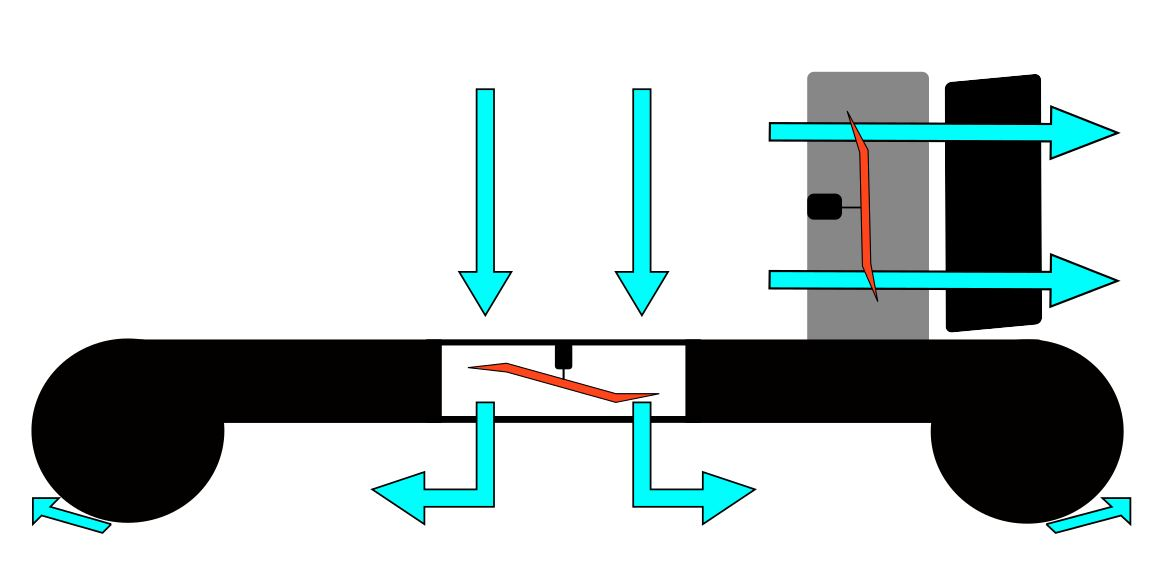
\includegraphics[width=0.8\textwidth]{Fotos/Funktionsprinzip.JPG}
  \caption{Funktionsprinzip eines Hovercrafts  \label{fig:Funktionsprinzip}}
\end{figure}